\title{Golf Practice Animation Report}
\author{}
\documentclass[a4paper,11pt]{article}
\usepackage[utf8]{inputenc}
\usepackage{pdfpages}
\usepackage{amssymb}
\usepackage{amsmath}
\usepackage{float}
\usepackage{siunitx}        % Provides the \SI{}{} and \si{} command for typesetting SI units
\usepackage{graphicx}       % Required for the inclusion of images
\usepackage[shortlabels]{enumitem}
\usepackage[T1]{fontenc}
\usepackage[a4paper, total={6in, 8in}, margin=25mm]{geometry} %margins
\usepackage{hyperref}
\hypersetup{colorlinks=true,linkcolor=black, citecolor=black}
\usepackage{tocloft}
\usepackage{lastpage}
\usepackage{fancyhdr}
\usepackage{subfig}
\pagestyle{fancy}
\renewcommand{\headrulewidth}{0pt}
\fancyhead{}
\lfoot{\fontsize{9}{9} \selectfont EMI Capstone Final Report (ENGR90038)\\ Copyright © Qionghui Cai, Yifan Xing, Zijie Yang, 2020}
\cfoot{\fontsize{9}{9} \selectfont \today}
\rfoot{\fontsize{9}{9} \selectfont Page \thepage \ of \pageref{LastPage}}


\makeatletter

\date{\today}               % Date for the report
\let\thetitle\@title        % Document title saved in command
\let\theauthor\@author      % Document author saved in command

\makeatletter
\g@addto@macro\@floatboxreset\centering
\makeatother
\renewcommand{\cftsecleader}{\cftdotfill{\cftdotsep}}

\usepackage{fontspec}
% Times New Roman
\setromanfont[
BoldFont=timesbd.ttf,
ItalicFont=timesi.ttf,
BoldItalicFont=timesbi.ttf,
]{times.ttf}
% Arial
\setsansfont[
BoldFont=arialbd.ttf,
ItalicFont=ariali.ttf,
BoldItalicFont=arialbi.ttf
]{arial.ttf}

\setlength{\parindent}{0pt}
\setlength{\parskip}{6pt}
\usepackage{changepage}

\usepackage{titlesec}

\titleformat*{\section}{\Large\bfseries\sffamily}
\titleformat*{\subsection}{\large\bfseries\sffamily}
\titleformat*{\subsubsection}{\normalsize\bfseries\sffamily}

\usepackage[]{xcolor}
\definecolor{melblue}{RGB}{31, 54, 90}
\definecolor{hrule}{RGB}{89, 128, 184}

\usepackage[style=apa]{biblatex}
\addbibresource{ref.bib}

\titlespacing*{\section}
{0pt}{0pt}{0pt}
\titlespacing*{\subsection}
{0pt}{0pt}{0pt}

\setlength{\belowcaptionskip}{-10pt}

\begin{document}

\begin{center}
    \includegraphics[width=3cm, height=3cm]{icon.png}
    \\[1cm]
    \fontsize{16}{16}\sffamily\bfseries\textcolor{melblue}{Golf Practice Animation}
    \vspace{5pt}
    \textcolor{hrule}\hrule
    \vspace{20pt}
    \color{black}\fontsize{11}{11}
    \bfseries\sffamily Qionghui Cai
    \\
    \mdseries\rmfamily 950415, qionghuic@student.unimelb.edu.au
    \\[1cm]
    \bfseries\sffamily Yifan Xing
    \\
    \mdseries\rmfamily 947930, yifxing@student.unimelb.edu.au
    \\[1cm]
    \bfseries\sffamily Zijie Yang
    \\
    \mdseries\rmfamily 825694, zijiey@student.unimelb.edu.au
    \\[1cm]

\end{center}

\begin{adjustwidth*}{1cm}{1cm}
\textbf{\textit{Executive Summary:}} \textit{Golf is becoming more popular as it becomes more urban and technological. Some amateur golfers, however, have difficulty improving their skills as they cannot clearly understand their shots. The aim of this project is to monitor a golfer’s shot result so that it can be displayed on any device, such as an iPhone or Android. This shot information includes speed, predicted trajectory, direction, peak, and carry, which can be used to correct the golfer’s swing in real- time. This project adopted a Doppler radar-based golf ball flight trajectory analysis system with a multi-platform visualisation mobile application. A variety of technologies in different fields, including radar hardware design, kinematic model prediction, wireless transmission and mobile application design are collaboratively utilised to construct a complete product.}
\end{adjustwidth*}
\vspace{\fill}

\thispagestyle{empty}
\newpage

\tableofcontents{\protect\thispagestyle{empty}}
\pagestyle{fancy}
\clearpage
\setcounter{page}{1}
\newpage



\section{Introduction}
In order to enable amateur golfers to enjoy real golf and improve their skills, this system is designed to help amateur golfers overcome the problem that hindering their improvement.
Technologies from multiple fields were adopted to develop this real-time golf flight trajectory visualization system. In this project, the use of new technologies in traditional sports has shown the development and prospects of using consumer electronics in traditional sports.

\begin{figure}[H]
    \centering
    \includegraphics[width=0.8\textwidth]{figure/BlockDiagram_bw.pdf}
    \caption{High-level block diagram of the system}
     \label{fig:block}
\end{figure}

The high-level block diagram of the system is shown in Figure \ref{fig:block}. This system is based on two IVS-565 radars. By using 24GHz Doppler radars with four antennas and a processing circuit including amplifier, filter, level shifter, power supply and ADC, real-time monitoring of the golf Doppler effect can be achieved. The multi-module back-end server equipped on the Raspberry Pi will automatically analyse the Doppler effect of the golf ball and calculate the golf launch speed and angle by adopting the phase-comparison monopulse method.
By deploying the kinematic model, the flight trajectory of the golf ball can be predicted. Finally, the system transmits the flight trajectory data to the smartphone through a transmission module based on Bluetooth low energy and compression algorithms. The easy-to-use visualization application provides the user with a multi-angle 3D golf flight trajectory for each shot.


\newpage
\section{Literature Review}
The existing mainstream simulator sensing devices are roughly divided into three types \textcite{tuxen2020method}.
the first one is the Infrared sensing system,it's Working principle is based on using infrared measurement system, and it has following advantages: Good durability, wide adaptability, low price, low maintenance cost, high cost performance.In a word, It is an affordable choice for experiencing the fun of golf indoors and suitable for entertainment environment.

The second trend is using High-speed camera sensor system, and this kind of devices are using split-type high-speed camera measurement system, Canadian industrial-grade surveillance camera equipment, binocular vision measurement and precise analysis.
its advantages are mainly utilised in accuracy , so it is more suitable for professional players. meanwhile, it is easy to use, and adaptable. Normally, it can accurately measure the flight data of 8 groups of golf balls,support swing action drawing line analysis, and has the most realistic stadium software system. So it is an excellent choice for players who want to improve their skills.

The last type is Radar sensing system.  The Working principle is  using radar detection system.
this devices have plenty of advantages like extremely professional golf tracking and testing equipment, \textcite{trackmangolf} with an accuracy of 0.3 yards per 100 yards, accurate data for 14 sets of golf balls, 9 sets of club data, 3 sets of measured data, and the measurement accuracy is approved by authoritative golf institutions such as Professional Golfers' Association (PGA) Certification; comes with swing analysis software,which can freely connect to terminal devices such as iPad, iPhone, PC. The most typical example is the Trackman radar measuring device, and it is currently widely used by PGA professional golfers and is a professional high-end choice for improving golf swing and hitting skills.





\newpage
\section{Hardware Design}
This chapter is mainly introducing the selection of hardware components and the design of each circuit. In section 3.1, it is including the overall structure of the hardware. Section 3.2 introduces the selection and design of the radar model. Considering the output signal of the initial radar circuit is undetectable and the condition of signal aliasing, Therefore, a suitable amplifying filter circuit is essential, so the main content of 3.3 is amplifier selection and amplifying filter circuit design. As for part 3.4, it is a cornerstone for further digital signal processing, which is explains the power supply circuit and DC level shifter design, all of this is contributing to an independent circuit which can go through ADC.
\subsection{Overall hardware architecture}
This section explains the overall hardware structure design of golf track detection system. In details, this system is divided into four 
44
 parts: radar circuit, amplifying and filtering circuit, power supply circuit, and DC level shifter circuit. Which is specifically illustrate in the Figure 2.
\begin{figure}[H]
    \centering
    \includegraphics[width=9cm,,height=11cm]{figure/hardware
    architecture.jpg}
    \caption{hardware architecture}
\end{figure}
This flowchart mainly focuses on processing analog signals. The reason for using two radar systems is to obtain both elevation angle and azimuth angle of the golf ball through different placement methods of the radar, and chapter 4 will concentrate on the algorithm of signal processing after going through the analog-to-digital converter.
\subsection{Radar}
Radar is an electromagnetic system emitting and receiving radio signals to detect and measure objects’ information within its detectable range. There are two main types of radar, pulse wave and continuous-wave(CW). Pulse radar will not send the next pulse until it completes each transmitting and receiving cycle. One antenna is enough to satisfy all operating requirements. On the contrary, CW radar needs one more antenna. Because it can emit a signal and receive another return signal at the same time. Compared with pulse wave radar, CW radar does better in the simplification of microwave filtering due to its narrower transmitted spectrum. Also, it can handle almost all objects with controllable speed at any distance (\cite{skolnik1970radar}). Considering these factors, CW radar is adopted in this project. 

 Doppler frequency refers to the change of frequency when an object moves along a direction due to the difference in its travel distance, showed as Figure \ref{fig:doppler} (\cite{DopplerRader}). One of the main pieces of information that can be extracted from the Doppler frequency is the radial velocity. The Doppler frequency becomes lower when the object is heading away from the radar with a smaller frequency return signal.
 \begin{figure}[H]
    \centering
    \includegraphics[width=10cm]{figure/Radar.png}
    \caption{Doppler Radar Principle}
    \label{fig:doppler}
\end{figure}
Doppler frequency f$_d$ can be expressed as
\begin{align}
    f_{d}=f_{r}-f_{t}
\end{align}
Where f$_r$ is the frequency of received signal and f$_t$ is the frequency of transmitting signal. When the receiver and sound source are close to each other, the receiving frequency is greater than the transmitting frequency. That is f$_d$ > 0. Otherwise, f$_d$ < 0.

The relationship between Doppler frequency and  radial velocity is 
\begin{align}
V_{r}=\frac{\lambda}{2} f_{d}=V \cos \theta
\end{align}


From the equations above, the following conclusions can be drawn.
\begin{itemize}[noitemsep,topsep=0pt]
   \item As long as the target Doppler frequency is measured, the velocity of the target can be obtained
   \item The Doppler shift of fixed target  shift is zero
   \item The positive and negative sign of the Doppler shift determine the direction of the target motion
\end{itemize}

In this project, the ideal radar model is IVS565, Section 3.2.1 is about the basic characteristics of the selected radar. Then Section 3.2.2 explains the reasons for choosing this type of radar. In Section 3.2.3, the main content is the connection and placement instructions of the radar circuit.
\subsubsection{IVS-565 Radar}
IVS 565 is a K-Band VCO radar transceiver for FMCW/FSK modulation from Innosent company. 
The Innosent company is established in 1999. It is a high-tech company specializing in the design ,production, sales. industrial, commercial, automatic control and other fields of radar sensors.
IVS-565 radars contains an advanced PHEMT -oscillator for lowest power consumption. It is also an Ideal device for security applications. 
\begin{figure}[H]
    \centering
    \includegraphics[width=6cm]{figure/IVS-565Radar.jpg}
    \caption{IVS-565 Radar}
    \label{png_IVS565}
\end{figure}
Meanwhile, It adopts a planar microstrip antenna structure and has a very small appearance. All of these characteristics make it suitable for various integrated circuits. IVS-565’s functions are also diverse, such as detecting the speed of objects and identifying the direction of moving targets.
\begin{figure}[H]
    \centering
    \includegraphics[width=8cm,height=6cm]{figure/IVS-565Structure.jpg}
    \caption{IVS-565 Structure}
\end{figure}
As for this project, the CW-mode has been chosen for IVS-565, its main theory is: According to the direction of movement of the object, the wave front transmitted by the wave generator (sound, microwave, light, etc.) is either "Compress" or "shrink", which ultimately means frequency changes. Signal shift in Initial frequency and reflection frequency from relatively unchanged transmitted signal are combined in the simple mixer (called "homodyne" by experts) , as a result, it produces sinusoidal intermediate products frequency (IF).
\subsubsection{Radar Selection}
The selection of Radar should fit into the condition that needs to apply for golf ball trajectory simulation. The requirements is to both detect angles and speed. The ability to detect both elevation angle and azimuth angle is the most tricky part. The existing technology can take advantages of phase differences of the returned signal to obtain angles.
A single pulse is transmitted by a directional antenna and received by two independent antennas. The distance between these antennas is known. The two antennas face the same direction and cover the same spatial area. The reflected signal has the same amplitude, resulting in a different phase.
Conversely, the angle θ of the object can be obtained by measuring the phase difference between the two signals. By placing another antenna on the left or right side of one of these antennas, the azimuth angle can be obtained. Meanwhile, putting one antenna above or lower than another antenna helps to calculate elevation angle.
\begin{figure}[H]
    \centering
    \includegraphics[width=6cm,height=6cm]{figure/phase comparison in angle determine .jpg}
    \caption{phase comparison in angle determine}
\end{figure}
So the distance d between two antennas is a crucial factor, If d is larger than the antenna diameter, high side lobes will be produced, which will result in wrong angle measurement . In order to limit the strength of the side lobes, the radar contains of two antennas will be the best choice for detecting angles.
Using above method, although IPM,IVS,IPS these three types of radar are all suitable for detecting objects, between them, IVS-565 is the most suitable for our project because it has two antennas to detect instantaneous speed, direction of movement, and instantaneous distance for moving objects. 
\subsubsection{Radar Circuit connection}
The CW-Doppler radar is the simpliest and most efficient solution in cases where the detection of moving object is the only and outstanding task. 
IVS-565 radar contains 6 pins, and the connection will be shown According to  \textcite{IVS-565}
the typical positive power supply is +5V, and the negative power supply in proper condition is -3.3V, meanwhile, decoupling capacitors are used to reduce noise from the equipment to the power supply. Considering the mode is CW, so the connection for Vtune is suspended. In this way, the transmit frequency will be set to the default value , which is 24 GHz at 25 C.
the remaining two output pin will be connect to the input of the amplifying filter circuit.
As for the placement, One of the radars obtains the azimuth angle through horizontal fixation
Another radar will fix the antenna vertically to obtain the elevation angle. Moreover, in order to make the angle detection more precisely, it is necessary to keep the centroids of the two radars at the same level. 
\subsection{Amplifying filter circuit design}
Combined with the condition that the output of IVS-565 is too small, amplifying circuit is needed for detection. Section 3.3.1’s content is covering the basic requirement for amplifying filter circuit, section 3.3.2 denotes the selection of the amplifier, and section 3.3.3 describes our circuit configuration and simulation results. At the end, considering the COVID-19, the project adjust another circuit to suit for reality.
\subsubsection{Design Requirements}
According to \textcite{IVS-565}, the output power is of IVS-565 almost 15.849mw, its too small, and in order for detecting the signal information, it is necessary to add further amplification circuit, the amount is in theory should be 70 to 80 dB from \textcite{Application_Note_I}
\begin{align}
\operatorname{gain}_{\max }=10^{\frac{80}{20}}=10000    
\end{align}
\begin{align}
\operatorname{gain}_{\min}=10^{\frac{70}{20}}=3162    
\end{align}
Meanwhile, due to the relationship between the moving objective and the output frequency:
\begin{align}
f_{\text {Dopp}}=2\cdot f_{0}\cdot\frac{v}{c_{0}}\cdot\cos \alpha
\end{align}
Where fdopp represents the Doppler frequency, and  f0 denotes the transmit frequency of the radar. v represents magnitude of velocity of the moving objects, and c0 is velocity of light, then alpha is the angle between the actual direction of motion and the connecting line sensor-object.
In general, choosing the angle between the golf ball and sensor to be 0, and the fastest golf ball speed is around 340km/h from \textcite{kobayashi1988golf},every golf players will impossible to hit the ball exceeding this speed, so this frequency of 15KHZ should be the upper limit for our filter, and the frequency beyond this value should be declined to remove the noise. Selecting 24 GHz as transmit frequency\textcite{Application_Note_I},
\begin{align}
f_{\text {Dopp}}=2\cdot f_{0}\cdot\frac{v}{c_{0}}\cdot\cos \alpha_{ }
\end{align}
\begin{align}
f_{\text {Dopp}}=2\cdot24\cdot10^{9} \cdot\frac{340\cdot \frac{10}{36}}{3\cdot10^{8}}\cdot1=15.111 \mathrm{kHZ}
\end{align}
 On the other hand , it also makes a sense to create the lower limit because we don’t want every movement to be detected, such as people walking speed, which is corresponding to 6.8km/h
 \begin{align}
f_{\text {Dopp}}=2\cdot24\cdot10^{9} \frac{6.8\cdot \frac{10}{36}}{3\cdot10^{8}}\cdot1=302 \mathrm{HZ}
\end{align}
\subsubsection{Amplifier selection}
OP27G is a precision operational amplifier combines low power consumption offset and low noise characteristics. Its offset as low as 25μV, maximum drift is 0.6μV/°C, OP27 is an ideal choice for precision instrument applications, which allows accurate high-gain amplification of low-level signals and provides excellent dynamic accuracy in high-speed data acquisition systems.
Considering the required magnification is large, and the effect is better if two amplifiers are connected in series, so in this project, choose one of the magnifications to be 100 and the other to be 60.
\begin{figure}[H]
    \centering
    \includegraphics[width=4cm,height=4cm]{figure/OP27Gpin.PNG}
    \caption{OP27G pin connection}
\end{figure}
Then the gain bandwidth of the amplifier should be greater than
 \begin{align}
G B W>\text { gain }\cdot\text { bandwidth }=100\cdot15.2\cdot 10^{3}=1.52 \mathrm{MHZ}
\end{align}
The GBW from OP27G datasheet is 8MHZ when gain is 100, and its totally affordable, so it is suitable for choosing.
\subsubsection{LTSpice simulation}
LTSpice has the high simulation performance (multi-core parallel computing can be used) and Convenient operation, which is very helpful with the habits of engineers who need to make a lot of adjustments and observations on the circuit, and the operation achieves a good balance in efficiency and Authenticity.
Above requirements contribute to the main plan for amplitude filter circuit.in this way, the project combines low-pass filter, high-pass filter and amplification circuit together.
\begin{figure}[H]
    \centering
    \includegraphics[width=0.8\textwidth]{figure/Amplifyingfiltercircuit.png}
     \caption{Amplifying filter circuit}
\end{figure}
When designing the circuit,the project selects Butterworth filters.
The characteristic of the Butterworth filter is that the frequency response curve in the pass band is flat to the maximum without fluctuations, while it gradually drops to zero in the stop band.The higher the filter order, the faster the amplitude attenuation in the stop band, in this circuit,the filter order is set to be 2, The attenuation rate of the second-order Butterworth filter is 12 decibels per octave.
Leting the damping ratio ζ to be 1, then write following equations. \\As for the first filter:
\begin{align}
K 1=-\frac{R_{5}}{R_{6}}=-100
\end{align}
\begin{align}
\frac{C_{3}}{C_{4}} \leq \zeta^{2}\cdot(1-K 1)
\end{align}
\begin{align}
f_{c}=\frac{1}{2 \pi \sqrt{R_{4} R_{5} C_{3} C_{4}}}=15.11 \mathrm{KHZ}
\end{align}
Considering electronic components available around, choose C3=100p, C4=0.022μ, then R6=270Ω, R5 =27kΩ, R4=1.8kΩ. \\ 
As for the second filter:
\begin{align}
K 2=-\frac{C_{1}}{C_{2}}=-68
\end{align}
\begin{align}
f_{c}=\frac{1}{2 \pi \sqrt{R_{1} R_{2} C_{2} C_{5}}}=302 \mathrm{HZ}
\end{align}
Considering the existing elements, choose C1=6.8μ, C2=0.1μ, C5=0.1μ, then R1=180Ω, R2=180kΩ.
After simulating,  The result is within the expected range.

\subsubsection{Real implementation}
This year due to the COVID-19, there is no way to go outside to complete the project, which also means given such a huge speed for radar to detect is impossible. So the plan about the amplification circuit is adjusted by changing the frequency range within 15HZ to 1KHZ, the range refers to the speed limitation that move people's hand towards radar, then when waving arms in front of the radar, it can also give the useful waveform to do signal processing.
\begin{figure}[H]
    \centering
    \includegraphics[width=0.8\textwidth]{figure/realamplifyingfiltercircuit.png}
    \caption{real amplifying filter circuit}
\end{figure}
\begin{align}
f_{c 1}=\frac{1}{2 \pi C_{3} R_{4}}=\frac{1}{2 \pi C_{5} R_{6}}=15.23 \mathrm{HZ}
\end{align}
\begin{align}
f_{c 2}=\frac{1}{2 \pi C_{1} R_{5}}=1 \mathrm{KHZ}
\end{align}

The double filters are trying to make the signal decline as much as possible beyond the frequency range we want, and the last RC high pass filter is to avoid signal aliasing. 
\subsection{Power supply circuit}
This step is to make further detection becomes more convenient and independent, from Figure \ref{fig:power_radar} during the radar circuit, it need -3.3 V and +5V to drive at a normal operation condition. Besides, active filter amplifier also need connected to ±5V, in this way, two power mode to produce electricity are chosen.
\begin{figure}[H]
    \centering
    \includegraphics[width=0.8\textwidth]{figure/powersupplyofIVS565Radar.png}
    \caption{power supply of IVS-565 Radar}
    \label{fig:power_radar}
\end{figure}
\begin{figure}[H]
    \centering
    \includegraphics[width=0.4\textwidth]{figure/powerAM2.png}
    \caption{power supply of IVS-565 Radar}
    \label{fig:power_radar}
\end{figure}
Each radar consists of two output, and each one output needs a filter amplifier to connect, so the power supply of each amplifier circuit can be seen from above.
The power for each voltage supply can be calculated:
\begin{align}
+5 V: 8\cdot(20.216+28.494)+35\cdot2\cdot5=739.68 m W<1 W
\end{align}
\begin{align}
-5 V: 8\cdot(20.216+28.494)=389.68 m W<1 W
\end{align}
\begin{align}
-3.3 V: 2\cdot1\cdot3.3=6.6 m W<1 W
\end{align}
According to the calculated power, the type of the power module can be selected K-CUT A0505S-1W and K-CUT A0503S-1W.

\begin{figure}[H]
    \centering
    \includegraphics[width=0.6\textwidth]{figure/powersupplycircuit.jpg}
    \caption{power supply of IVS-565 Radar}
    \label{fig:power_radar}
\end{figure}

For circuits with strict noise requirements, additional circuits with LC parallel are used, and the value of capacitor and inductor is determined by Vin and Vout.
\subsection{ADC}
MCP3008 is 10-bit successive approximation ADC, mainly composed of input channel gate switch, sampling and holding unit, data converter (DAC), comparator, 10-bit successive approximation register (SAR), control logic unit and shift register, showed as Figure \ref{fig:ADC} (\cite{mcp3008}). The comparator compares the measured voltage with the known standard voltage. When the measured voltage equals to the standard voltage, the standard voltage is the result of A/D conversion. Standard voltage can be variable according to the binary code change, which is usually produced by the SAR and DAC. First it is produced by generating a binary encoding digital signal using SAR and this signal will be converted into analog voltage using DAC. The bits of SAR determines the resolution of A/D converter and the number of comparisons needed to complete an A/D conversion process. The channel number for each A/D conversion is selected by the control logic, and the converted binary data is serialized through the shift register (\cite{ADConverter}).
\begin{figure}[H]
    \centering
    \includegraphics[width=7cm]{figure/ADC.png}
    \caption{MCP3008 Functional Module}
    \label{fig:ADC}
\end{figure}
A 10-bit ADC represents an analog voltage expressed as a 10-digit number on the output. For example, if the analog voltage is measuring 0-3.3V, each step in the output value means 
\begin{align}
 3.3V /2^{10} = 3.3/1024 = 0.003V   
\end{align}
A 10-digit number multiplied by a step voltage of 0.003 represents the output voltage.
\subsubsection{DC-level shifting circuit}
The former radar circuit usually causes voltage offset of ±300mV, but the plan is to connect Analog-digital-converter to better process the signal information. The ADC of the project is MCP3008:

From the datasheet\textcite{mcp3008},the voltage range coming into MCP3008 needs to be 0-3.3V, but due to original negative offset of radar output, a voltage shifter circuit is necessary to better compensate the offset of the signal.

The level shifting circuit requires one amplifier, but there is no need for it to amplify the signal anymore, so just make  R7=R8
\begin{figure}[H]
    \centering
    \includegraphics[width=0.8\textwidth]{figure/level shifting circuit.png}
    \caption{power supply of IVS-565 Radar}
    \label{fig:power_radar}
\end{figure}

\begin{align}
V_{A}=V_{B}=\frac{R_{11}}{R_{10}+R_{11}}\cdot-5
\end{align}
\begin{align}
\frac{V_{i n}-V_{B}}{R_{7}}=-\frac{V_{c}-V_{B}}{R_{8}}
\end{align}

As a result, R8=150, R7=150, R11=20, R10=51k.


\newpage
\section{Trajectory Simulation Model}
This chapter introduces the main theory about how to extract interested information and use these information to build the prediction model. Section 4.1 illustrates the main components of kinematic model, including gravity, air resistance, Magnus force and buoyancy. Section 4.2 and Section 4.3 talk about acquiring the golf's flying velocity and angle respectively. Section 4.4 shows the mathematics deviation of trajectory simulation based on kinematic model.
\subsection{Kinematic Model}
The flying golf ball is mainly affected by gravity, drag force from air resistance, Magnus force and buoyancy, showed as Figure \ref{fig:model} (\cite{KinematicModel}). 
\begin{figure}[H]
    \centering
    \includegraphics[width=10cm]{figure/force.png}
    \caption{Kinematics Model of the flying ball}
    \label{fig:model}
\end{figure}
Gravity is caused by the attraction force of the earth, always with a direction going straight down. It can be defined by the equation:
\begin{align}
F_{g}=m g
\end{align}
where m is the mass of golf,kg; g is gravitational acceleration, 9.8m/s$^2$.\\

When the golf is flying, its surrounding air exerts a drag on it to push it back, opposite to the direction of velocity. This drag force has a nonlinear relationship with the velocity.
\begin{align}
\vec{F}_{d}=-\frac{1}{2} C_{D} \rho A v^{2} \frac{\vec{v}}{|v|}
\end{align}
where C$_D$ is the drag coefficient, with a common value 0.4. $\rho$ is air density, equaling to 1.23kg/m $^3$. A is the cross section area of the ball, related to the diameter of golf ball. Typically, the diameter of golf is 42.67mm\\

The golf ball rotates continuously around its own axis during its flight. When a fluid flows in the direction perpendicular to this axis, it will be subjected to a transverse force perpendicular to the direction of flow, which is called Magnus force, showed as Figure \ref{fig:magnus}.
\begin{figure}[H]
    \centering
    \includegraphics[width=8cm]{figure/Magnus.png}
    \caption{Magnus Force}
    \label{fig:magnus}
\end{figure}
It is determined by the golf's surface geometry,velocity,direction and spin rate. The mathematical expression is:
\begin{align}
    \vec{F}_{M}=\frac{1}{2} C_{L} \rho A v^{2}(\hat{\omega} \times \hat{v})
\end{align}
Where C$_L$ is the lift coefficient.

\subsection{Velocity Measurement}
Assume the flying object is R distance away from the receiving antennas. The numbers of wavelength corresponding to the distance back and forth is:
\begin{align}
n=\frac{2 R}{\lambda}    
\end{align}
Wavelength is define as:
\begin{align}
\lambda=\frac{c}{f_{t}}
\end{align}
Where $c=3 \times 10^{8} ; f_{t}=24 G H z$in this project\\
Since a wavelength means a 2 $\pi$ phase transformation. The total phase change is:
\begin{align}
\phi=2 \pi\left(\frac{2 R}{\lambda}\right)=4 \pi R / \lambda
\end{align}
The angular frequency refers to the rate of phase change when distance R varies over time. That is:
\begin{align}
\omega_{d}=\frac{d \phi}{d t}=\frac{4 \pi}{\lambda} \frac{d R}{d t}=\frac{4 \pi V_{r}}{\lambda}=2 \pi f_{d}
\end{align}
where $V_{r}=d R / d t$ and $f_{d}$ is Doppler frequency.\\
Rearrange the above equation, we get:
\begin{align}
V_{r}=\frac{\lambda}{2} f_{d}=V \cos \Theta
\end{align}
The velocity shown above is the radial velocity with angle $\theta$ with respect to the ground. Since the most critical value we need is the initial velocity infinitely approaching the swing point. The angle $\theta$ can be considered as 0 degree (\cite{martin2012evaluation}). That is:
\begin{align}
V=\frac{\lambda}{2} f_{d}
\end{align}


\subsection{Angle Measurement}
The main method being used to get angle is phase comparison method, showed as Figure \ref{fig:phase}, two antennas in the same direction separated by l meter receive the same ratio signal transmitting through directive antenna. The return signals received have same amplitude but different phases (\cite{li2015simulation}).
\begin{figure}[H]
    \centering
    \includegraphics[width=8cm]{figure/phase.png}
    \caption{Phase Comparison Method}
    \label{fig:phase}
\end{figure}
Distance difference from two receiver to the flying golf is:
\begin{align}
    \Delta R=R_{1}-R_{2}=l \sin \theta
\end{align}
Take the earth ground as the horizontal line. Assume the flying direction of the target is $\theta$, the phase difference should be:
\begin{align}
\Delta \varphi=\frac{2 \pi}{\lambda} \Delta R=\frac{2 \pi l \sin \theta}{\lambda}
\end{align}
Then, the angle can be expressed as:
\begin{align}
 \theta=\arcsin \frac{\lambda \Delta \phi}{2 \pi l}   
\end{align}

\subsection{Mathematic Model}
Velocity is decomposed into x,y and z axis.
\begin{align}
\begin{split}
    V_{x}&=V \cdot \cos \alpha \cdot \cos \theta\\
    V_{z}&=V \cdot \cos \alpha \cdot \sin \theta\\
    V_{y}&=V \cdot \sin \theta    
\end{split}
\end{align}
According to the kinematic model and Newton’s second law, analyse the force from x axis , y axis and z axis respectively. In this project, gravity and drag force due to the air resistance are the main factors to consider (\cite{AirResistanceModels}).\\

x axis:\\
when $v_{x 0}>0$
\begin{align}
    m \frac{\partial^{2} x}{\partial t^{2}}=-k\left(\frac{\partial x}{\partial t}\right)^{2}
    \label{1}
\end{align}
The initial conditions of above equations are:
\begin{align}
    \left.x\right|_{t=0}=0,\ \left.v_{x}\right|_{t=0}=v_{x 0}
\end{align}
where t is the flying time, s; k is the friction coefficient between the golf and air.

Substituting $v_{x}=\frac{\partial x}{\partial t}$ into equation (\ref{1}), we have:
\begin{align}
    m \frac{\partial v_{x}}{\partial t}=-k v_{x}^{2}
\label{2}
\end{align}
Separate the variable V$_x$ from the equation (\ref{2}) and integrate both sides of this equation. Also, apply the initial condition $\left.v_{x}\right|_{t=0}=v_{x 0}$. The analytic solution of this partial differential equation is:
\begin{align}
    v_{x}=\frac{m v_{x 0}}{m+k v_{x 0} t}
\end{align}
Again, separate the variable x and apply the initial conditions $\left.x\right|_{t=0}=0$.
\begin{align}
    x=\frac{m}{k} \ln \left(1+\frac{k v_{x 0} t}{m}\right)+x_{0}
\end{align}
When $v_{x 0}<0$
\begin{align}
    m \frac{d v_{x}}{d t}=k v_{x}^{2}
    \label{3}
\end{align}
Integrate equation (\ref{3}):
\begin{align}
    v_{x}=\frac{v_{x 0} m}{m-k v_{x 0} t}
    \label{4}
\end{align}
Integrate equation (\ref{4}):
\begin{align}
x=\frac{-m}{k} \ln \left(1-\frac{k v_{x 0} t}{m}\right)+x_{0}
\end{align}
z axis:\\
when $v_{z 0}>0$
\begin{align}
    m \frac{\partial^{2} z}{\partial t^{2}}=-k\left(\frac{\partial z}{\partial t}\right)^{2}\\
\end{align}
Separate the variable V$_z$ from the above equation and integrate both sides of this equation.
\begin{align}
    v_{z}=\frac{m v_{z 0}}{k v_{z 0} t+m}    
\end{align}
Again, separate the variable z and apply the initial conditions $\left.z\right|_{t=0}=0$.
\begin{align}
     z=\frac{m}{k} \ln \left(1+\frac{k v_{z 0} t}{m}\right)+z_{0}   
\end{align}
When $v_{z 0}<0$
\begin{align}
    v_{z}=\frac{v_{z 0} m}{m-k v_{z 0} t}
\end{align}
Similarly,
\begin{align}
    z=\frac{-m}{k} \ln \left(1-\frac{k v_{z 0} t}{m}\right)+z_{0}
\end{align}
Where the initial conditions are:
\begin{align}
    \left.z\right|_{t=0}=0,\left.v_{z}\right|_{t=0}=v_{z 0}
\end{align}

y axis:\\
The vertical y axis is influenced by gravity and air resistance. According to the kinematic model and Newton’s second law:
\begin{align}
\begin{split}
   m \frac{\partial^{2} y}{\partial t^{2}}&=-k\left(\frac{\partial y}{\partial t}\right)^{2}-m g\qquad(\frac{\partial y}{\partial t} \geq 0)\\
   m \frac{\partial^{2} y}{\partial t^{2}}&=k\left(\frac{\partial y}{\partial t}\right)^{2}-m g\qquad(\frac{\partial y}{\partial t} \leq 0)
\end{split}
\end{align}
Where the initial conditions are:
\begin{align}
    \left.y\right|_{t=0}=h,\left.v_{y}\right|_{t=0}=v_{0 y}
\end{align}
Substituting $v_{y}=\frac{\partial y}{\partial t}$t into equation $m \frac{\partial^{2} y}{\partial t^{2}}=-k\left(\frac{\partial y}{\partial t}\right)^{2}-m g$, we have:
\begin{align}
    m \frac{\partial v_{y}}{\partial t}=-k v_{y}^{2}-m g
\end{align}
Adopting the method of separating variables and apply the initial condition $\left.v_{y}\right|_{t=0}=v_{y 0}$.
\begin{align}
    v_{y}=\sqrt{\frac{m g}{k}} \tan \left[\arctan \left(\sqrt{\frac{k}{m g}} v_{y 0}\right)-t \sqrt{\frac{g k}{m}}\right]
\end{align}
Again, separate the variable x and apply the initial conditions $\left.y\right|_{t=0}=h$.
\begin{align}
    y=h-\frac{m}{k} \ln \left[\frac{\cos \left[\arctan \left(\sqrt{\frac{k}{m g}} v_{y 0}\right)\right]}{\cos \left[\arctan \left(\sqrt{\frac{k}{m g}} v_{y 0}\right)-t \sqrt{\frac{g k}{m}}\right.}\right]
\end{align}
When $v_{y}=0$, the golf reaches the highest position. That is:
\begin{align}
    t=t_{1}=\sqrt{\frac{m}{g k}} \arctan \left(\sqrt{\frac{k}{m g}} v_{y 0}\right)
\end{align}
\begin{align}
    y_{\max }=h-\frac{m}{k} \ln \left\{\cos \left[\arctan \left(\sqrt{\frac{k}{m g}} v_{y 0}\right)\right]\right\}
\end{align}
When $t>t 1$, the golf begins to fall.
\begin{align}
    v_{y}=\frac{\sqrt{\frac{m g}{k}}\left(1-e^{\sqrt{\frac{k g}{m}}\left(t-t_{1}\right)}\right)}{1+e^{\sqrt{\frac{k g}{m}}\left(t-t_{1}\right)}}
\end{align}
\begin{align}
    y=y_{\max }+\frac{m}{k} \ln \left\{\frac{4 e^{\sqrt{\frac{k g}{m}}\left(t-t_{1}\right)}}{\left[1+e^{\sqrt{\frac{k g}{m}}\left(t-t_{1}\right)}\right]^{2}}\right\}
\end{align}
When the golf ball hits the ground,y=0,substituting it into equation (34), the total flying time can be gotten:
\begin{align}
    T=t_{1}+\sqrt{\frac{m}{k g}} \ln \left(\frac{2-e^{-\frac{k}{m} y_{\max }}+2 \sqrt{1-e^{-\frac{k}{m} y_{\max }}}}{e^{-\frac{k}{m} y_{\max }}}\right)
\end{align}

\newpage
\section{Software design}
The back-end software of the project runs on a single board computer (Raspberry Pi 4). The front-end software of the project is designed to run on mainstream operating systems or platforms such as iOS, Android, Windows and macOS. Through the modular design, each module can be developed using the most suitable programming language to achieve the best development efficiency and maintainability. About three thousand lines of code, including C, Python and C\# constitute the software part of the project. The software design of this project needs to have the following functions: 
\begin{itemize}[noitemsep,topsep=0pt]
   \item Read ADC data through SPI protocol
   \item Analyse the radar data to get the launch speed and angle of the ball
   \item Compute the flight trajectory of the golf ball from the launch speed and angle
   \item Display flight trajectory on any supported front-end device
\end{itemize}
   
Ideally, the back-end system is designed to run automatically without user action after the power is turned on. The front-end system needs to have an easy-to-use graphic user interface for users to operate.



\subsection{Software Architecture}
The back-end server of this project is based on Raspberry Pi OS (formerly Raspbian), which is a Debian derivative for Raspberry Pi. The stability and large open-source community of Debian bring convenience to the project development. The front-end application is based on the Unity 3D engine. This engine was selected because of its cross-platform portability.
\par
Due to the impact of the epidemic, the communication and cooperation of the project team are affected by the level 3 restrictions and time difference. Through object-oriented programming, different modules can be assigned to different team members. By deploying Git for version control, different team members will not affect each other when editing code. The modular design of the project follows the design concept of high cohesion and low coupling program, the data exchange between modules is reduced to a minimum, and each module contains all the functions of its part.
\begin{figure}[H]
    \centering
    \includegraphics[width=\textwidth]{figure/Software.pdf}
    \caption{Software architecture diagram}
    \label{fig:software_diagram}
\end{figure}
The software architecture diagram is shown in Figure \ref{fig:software_diagram}. The main program of the back-end server is written in Python, it contains three modules. The data reading module is responsible for operating the ADC. The signal processing module is used to compute the flight trajectory from the radar signal. The transmission module is responsible for communicating with the front-end device. The front-end application scripts are written in C\#, it contains two modules. The transmission module communicates with the back-end server, and the visualisation module displays the flight trajectory on the user interface.


\subsection{ADC Reading}
The back-end server communicates with the ADC through the SPI protocol. According to the datasheet  \textcite{raspberrypi}, there are 4 SPI buses natively provided by its CPU (BCM2711) with maximum baud rates of 250MHz. 
\par
There are some open-source MCP3008 drivers with Python API or C API available for Raspberry Pi. As mentioned in the hardware section, the ADC sampling rate needs to reach 20ksps to meet the requirements of Nyquist theorem. Since most of the SPI drivers are dependent on the Linux kernel SPI driver, the speed limit of the Linux SPI driver may limit the final sampling rate.
\par
As shown in the Figure \ref{fig:spi}, by testing the driver at different baud rates, the lowest baud rate required by the project can be obtained. When the baud rate is higher than 4MHz, the sampling speed of the Linux SPI driver can meet the requirement of 20ksps.
\begin{figure}[H]
    \centering
    \includegraphics[width=0.6\textwidth]{figure/spi_linux.pdf}
    \caption{Linux SPI driver speed test}
    \label{fig:spi}
\end{figure}
In addition to the impact of the Linux driver, the clock accuracy of a programming language may also affect the accuracy of the sampling period. The sampling period of ADC in this project $ 1/20ksps=0.00005s=0.05ms$. As a high-level programming language, the accuracy of Python’s clock module will be affected by many factors. According to \textcite{python}, the time module of Python can only guarantee millisecond precise, and the specific value of accuracy depends on the operating system. Therefore, the ADC reading module needs to be independent of the main program and written in C.
\par
\textcite{pigiop} is an open-source C library for Raspberry Pi to control General Purpose Input Outputs (GPIO). The SPI wrapper API provided by the pigpio library can meet the requirements for both ADC sampling rate and sampling period accuracy.
\par
The simplified finite state machine (FSM) of the ADC reading module is shown in Figure \ref{fig:adc_module}. When the main program calls the ADC reading module, the module will enter the detection state. In the detection state, the module will read ADC values at a speed of 1ksps. When two or more of the four ADC channels reach the corresponding high voltage threshold, the module will enter the sampling state. In the sampling state, the ADC reading module will sample and store the ADC value at a speed of 20ksps. When two or more channels are lower than the corresponding low voltage threshold, the module will return the data to the main program. Due to the radar signal characteristics mentioned in the hardware section, each channel will have a different voltage threshold.
\begin{figure}[H]
    \centering
    \includegraphics[width=0.5\textwidth]{figure/SPI.pdf}
    \caption{FSM of the ADC reading module}
    \label{fig:adc_module}
\end{figure}
Since the ADC module is written in C, the module needs to be compiled into a dynamically linked shared object library (.so) and imported by the ctypes module of Python.



\subsection{Signal Processing}
The Doppler Effect of CW radars can be used to calculate the velocity of the golf. When there is relative motion between the emission signal and the received signal, the received signal frequency will be different from the emission signal frequency. That is, the Doppler frequency shift is not zero. If the golf is moving close to the radar, the received echo frequency is higher than the transmitting frequency. The Doppler frequency is positive, but negative on the contrary. The relationship between them is: 
\begin{align}
V_{r}=\frac{\lambda}{2} f_{d}=V \cos \theta
\end{align}

In this project, a special 3-dimensions coordinate system with three axes is adopted. X axis represents the left and right space. Z axis represents the front and back space. Y axis represents the up and down space. In this way, the position of the flying ball will involve two angles. One is called azimuth $\theta$ related to x and z axes. The other one is called elevation $\alpha$, the angle between the golf and the horizon, showed as Figure \ref{fig:angle}.
\begin{figure}[H]
    \centering
    \includegraphics[width=10cm]{figure/Angle.png}
    \caption{Azimuth and Elevation}
    \label{fig:angle}
\end{figure}
Double radar systems with two antennas are being used. One of the radar is placed horizontally to get the azimuth. And the other one is placed vertically to obtain the elevation. The return signal received by the two antennas in every radar has the same amplitude and different phase, showed as Figure \ref{fig:PD}. Like discussed in section 4.3, once the phase difference is obtained, the angle can be obtained by: 
\begin{align}
 \theta=\arcsin \frac{\lambda \Delta \phi}{2 \pi l}   
\end{align}
\begin{figure}[H]
    \centering
    \includegraphics[width=10cm]{figure/Phase3.png}
    \caption{Phase Difference}
    \label{fig:PD}
\end{figure}
\subsection{Trajectory Simulation}
The flying golf ball is mainly affected by gravity, drag force from air resistance, Magnus force and buoyancy, showed as Figure \ref{fig:model2} (\cite{martin2012evaluation}). 
\begin{figure}[H]
    \centering
    \includegraphics[width=8cm]{figure/KM.png}
    \caption{Kinematics Model of the flying ball}
    \label{fig:model2}
\end{figure}
Among them, the strength of Magnus force is related to the rotational speed, difficult to be measured. The magnitude of the buoyancy is two orders smaller than the gravity and drag force, which is usually can be neglected. In this project, the effect of gravity and drag force from air resistance are mainly taken into account. According the kinematic model, the position at t moment of the flying golf can be obtained as follow.

The x position at t moment is given by:
\begin{align}
\begin{split}
  x=\frac{m}{k} \ln \left(1+\frac{k v_{x 0} t}{m}\right)+x_{0} \qquad(v_{x 0}>0)\\ 
  x=\frac{-m}{k} \ln \left(1-\frac{k v_{x 0} t}{m}\right)+x_{0} \qquad(v_{x 0}<0)
\end{split}
\end{align}

The z position at t moment is given by:
\begin{align}
\begin{split}
 z=\frac{m}{k} \ln \left(1+\frac{k v_{z 0} t}{m}\right)+z_{0}  \qquad(v_{z 0}>0)\\ 
z=\frac{-m}{k} \ln \left(1-\frac{k v_{z 0} t}{m}\right)+z_{0} \qquad(v_{z 0}<0)
\end{split}
\end{align}

The y position at t moment is given by:
\begin{align}
    t=t_{1}=\sqrt{\frac{m}{g k}} \arctan \left(\sqrt{\frac{k}{m g}} v_{y 0}\right)
\end{align}
\begin{align}
    y_{\max }=h-\frac{m}{k} \ln \left\{\cos \left[\arctan \left(\sqrt{\frac{k}{m g}} v_{y 0}\right)\right]\right\}
\end{align}
\begin{align}
\begin{split}
   y=h-\frac{m}{k} \ln \left[\frac{\cos \left[\arctan \left(\sqrt{\frac{k}{m g}} v_{y 0}\right)\right]}{\cos \left[\arctan \left(\sqrt{\frac{k}{m g}} v_{y 0}\right)-t \sqrt{\frac{g k}{m}}\right.}\right] \qquad(t<t_1)\\
    y=y_{\max }+\frac{m}{k} \ln \left\{\frac{4 e^{\sqrt{\frac{k g}{m}}\left(t-t_{1}\right)}}{\left[1+e^{\sqrt{\frac{k g}{m}}\left(t-t_{1}\right)}\right]^{2}}\right\}\qquad(t>t_1)
\end{split}
\end{align}

\subsection{Wireless Communication}
In order to make the front-end application works on different platforms, the wireless protocol used for this project needs to be a common protocol that is widely used in consumer electronic devices. The Bluetooth protocol is a universal protocol that is easy to develop and easy to use. Due to the limitation of iOS on the classic Bluetooth protocol, the Bluetooth Low Energy protocol was finally adopted as an alternative.


\subsubsection{BlueZ}
Since there is no mature Bluetooth Python wrapper solution on Linux, the transmission module of this project directly calls BlueZ to establish connections without using Python wrappers. \textcite{bluez} is a Bluetooth stack included in the Linux kernel. the Bluetooth daemon process works as the Bluetooth control centre and handles Bluetooth-related tasks. BlueZ provides the implementation of the Bluetooth communication protocol and interface. It uses \textcite{dbus} to communicate with other processes and provides APIs for Python while controlling the Bluetooth daemon as shown in Figure \ref{fig:bluez}. Therefore, the main program process of the back-end server does not need to access the Bluetooth daemon directly. The transmission module only needs to implement access to the D-Bus interface of BlueZ for controlling Bluetooth.
\begin{figure}[H]
    \centering
    \includegraphics[width=0.6\textwidth]{figure/bluez.pdf}
    \caption{Bluez D-Bus architecture}
    \label{fig:bluez}
\end{figure}


\subsubsection{Bluetooth Low Energy Protocol}
According to \textcite{bluetooth}, Bluetooth Low Energy (BLE) is a low-power and low-cost transmission technical specification integrated with Bluetooth 4.0. It defines some profiles to describe how a device works in a specific scenario. Generic Attribute Profile (GATT) is a type of profile defined by BLE. It is built on top of the Attribute Protocol (ATT) and establishes some common operations and frameworks for the transmitted data in the attribute protocol.
\par
According to the GATT specification in \textcite{bluetooth}, a profile is constructed by one or more services, and service describes one or more characteristic as shown in Figure \ref{fig:gatt} from \textcite{ble}. In the transmission module of the project, \textcite{nus} is used to implement a service that emulates a serial port, more specifically the Universal Asynchronous Receiver/Transmitter (UART). This service includes a read-only channel (RX) for transmitting trajectory data and a write-only channel (TX) for transmitting feedback from the front-end. 
\begin{figure}[H]
    \centering
    \includegraphics[width=0.3\textwidth]{figure/gatt.jpg}
    \caption{GATT profile hierarchy}
    \label{fig:gatt}
\end{figure}


Generic Access Profile (GAP) is a specification used by GATT to control devices for connection and broadcast. As mentioned in \textcite{ble}, before the devices establish GATT connections and exchanges data, they need to be first connected through the Generic Access Profile (GAP). GAP defines devices as peripheral devices and central devices as shown in Figure \ref{fig:broadcast} from \textcite{ble}. Peripheral devices keep broadcasting data to surrounding devices at a fixed frequency. The central device scans the surroundings peripheral device and requests scan response from the scanned peripheral. When the peripheral receives the scan response request, it will send the required data to the central device as illustrated in Figure \ref{fig:advertise} from \textcite{ble}.
\begin{figure}[H]
    \centering
    \includegraphics[width=0.6\textwidth]{figure/broadcast.jpg}
    \caption{BLE Broadcasting topology}
    \label{fig:broadcast}
\end{figure}
\begin{figure}[H]
    \centering
    \includegraphics[width=\textwidth]{figure/advertise.jpg}
    \caption{GAP advertising process}
    \label{fig:advertise}
\end{figure}


In this project, the back-end server operates as a peripheral device and broadcasts to surrounding devices through GAP while maintaining low power consumption. When the user opens the front-end application in the smartphone or other central devices, it automatically searches for surrounding back-end server and establishes a GATT connection. Finally, the trajectory data will be sent to the front end through the RX channel after each 
shot.

As can be seen from Figure \ref{fig:nus}, after NUS is advertised, the front-end device will automatically establish a GAP connection and start GATT. The NUS established by the transmission module contains two UART channels, RX and TX.
\begin{figure}[H]
    \centering
    \includegraphics[width=0.5\textwidth]{figure/nus.png}
    \caption{NUS of the transmission module}
    \label{fig:nus}
\end{figure}

\subsubsection{Data Compression}
Since GATT has a limitation of the maximum transmission unit (MTU) according to Bluetooth, trajectory data must be fragmented to be transmitted. As demonstrated in Figure \ref{fig:mtu}, the MTU of the transmission module is 517 bytes. This value was obtained using nRF Connect, which is a BLE testing tool provided by Nordic Semiconductor.
\begin{figure}[H]
    \centering
    \includegraphics[width=0.5\textwidth]{figure/mtu.png}
    \caption{MTU of the transmission module}
    \label{fig:mtu}
\end{figure}
To reduce transmission time, a simple compression module based on gzip was adopted since gzip is natively supported by Python and C\#. \textcite{gzip} is a compression tool based on Lempel–Ziv coding (LZ77). In the case of transmitting trajectory data, the size and the number of fragments of test data reduced to 40\% of the original data as shown in Figure \ref{fig:compress}. Transmission speed and stability have been greatly improved by the compression module.
\begin{figure}[H]
    \centering
    \includegraphics[width=0.7\textwidth]{figure/compression.pdf}
    \caption{Compression result}
    \label{fig:compress}
\end{figure}


\subsection{Visualization}
The front-end application is based on the Unity 3D engine with C\# scripting API. As mentioned in \textcite{unity}, Unity is a cross-platform game engine widely adopted in the area including video game, film and architecture. By adopting the unity engine, it becomes possible to develop an easy-to-use and beautiful graphical interface. The cross-platform nature of this engine enables the front-end application to be compiled to different platforms including iOS, Android, Windows and macOS after simple configuration. The wide use of Unity in the industry has also brought a large number of third-party plug-ins and materials, which has dramatically accelerated the development process of the project. The transmission module of the front-end application is written using the C\# API of Unity to achieve platform independence.

\newpage
\section{Results \& Analysis}
\subsection{Hardware results and analysis}
\begin{figure}[H]
    \centering
    \includegraphics[width=0.8\textwidth]{figure/Hardware Appearance.jpg}
    \caption{Amplifying filter simulation result}
     \label{fig:hardware}
\end{figure}
The Figure \ref{fig:hardware} contains all the hardware circuit we implemented in the reality,once the radar detect any moving object, the signals represented by various frequency wareforms will go though the amplifying process, adding filter to avoid aliasing and power supply to drive, then successfully transmit the analog signal to digital information across ADC.
\subsubsection{Amplifying filter circuit results analysis}
\begin{figure}[H]
    \centering
    \includegraphics[width=0.8\textwidth]{figure/Amplifyingfiltersimulation result.png}
    \caption{Amplifying filter simulation result}
     \label{fig:amplifying}
\end{figure}
As shown in Figure \ref{fig:amplifying}, aiming for detecting the golf ball speed, the amplifier frequency range is successfully within the period of 230HZ to 13.3KHZ, and the amplifying amount is also between 70dB and 80dB.
\begin{figure}[H]
    \centering
    \includegraphics[width=0.8\textwidth]{figure/realamplifyingfiltersimulationresult.png}
    \caption{real amplifying filter simulation result}
     \label{fig:amplifying_real}
\end{figure}
Referring of the COVID-19 restriction, which is the realistic goal for detecting people waving the hand, the amplifier frequency range is successfully adjusted within the period of 15HZ to 1KHZ in Figure\ref{fig:amplifying_real}. 
\begin{figure}[H]
    \centering
    \includegraphics[width=0.8\textwidth]{figure/radar output results1.png}
    \caption{radar output results1}
     \label{fig:radar_output}
\end{figure}
Figure\ref{fig:radar_output} is the realistic radar output results, as it is shown, the two radar output will stay in a steady state until a moving objects is into its detective zone, and the The closer people are to the radar sensor, the amplitude of the output wave will become larger. Instead of the golf ball, hands become the object, swing hands the faster, the larger frequency of the output waveform will have.
In addition, the two actual waveforms of the radar output are consistent with the theory calculated. The two waveforms are in the same size because the arm swings at only one speed. The phase difference is due to the different distance between the detected object and the antenna. At the same time, the phase difference is analyzed to obtain angle.

\subsubsection{DC-level shifting circuit results analysis}
\begin{figure}[H]
\centering
\includegraphics[width=0.8\textwidth]{figure/real output of radar signal.png}
\caption{real output of radar signal}
\label{fig:radar1}
\end{figure}
Figure \ref{fig:radar1} shows the radar output, the positive and negative offset is due to the radar inside circuit, the aim of level shifting is to make the wave voltage range all within 0 to 3.3V.
\begin{figure}[H]
\centering
\includegraphics[width=0.8\textwidth]{figure/level shifting simulation result.png}
\caption{level shifting simulation result}
\label{fig:SHIFT}
\end{figure}
The results shown on Figure \ref{fig:radar1} completely prove the effect of the level-shifting circuit, the negative offset can be move upper to above 0V.

\subsection{Matlab Simulation}
In this part,the kinematic model is implemented using Matlab to check  the accuracy of model. The simulation result is showed as Figure \ref{fig:matlab}, respectively showing the complete movement trajectory of golf and the prediction results of top view and side view.
\begin{figure}[H]
    \centering
    \includegraphics[width=\textwidth]{figure/Matlab.jpg}
    \caption{Trajectory Simulation in Matlab}
    \label{fig:matlab}
\end{figure}
The prediction results and error statistics of 20 sets of data are showed as Table \ref{5}. The initial values are (Initial velocity/MPH, elevation/degree,Azimuth/degree).
\begin{table}[H]
\caption{Prediction Error}
\label{5}
\begin{tabular}{|c|c|c|c|c|}
\hline
Index & Initial Value     & \begin{tabular}[c]{@{}c@{}}Reference \\ (Carry,Peak)\end{tabular} & \begin{tabular}[c]{@{}c@{}}Predicted \\ (Carry,Peak)\end{tabular} & \begin{tabular}[c]{@{}c@{}}Errors\\ (Carry,Peak)\end{tabular} \\ \hline
1     & (111.7,19.4,-1.9) & (156,33) & (144.32,30.77) & (-11.68,2.23) \\ \hline
2     & (102.6,19.5,1.6)  & (142,27) & (134.11,25.80) & (-7.89,-1.20) \\ \hline
3     & (103.9,25.4,-2.3) & (141,35) & (135.67,33.62) & (-6.67,-1.38)  \\ \hline
4     & (108.7,21.9,2.4)  & (150,34) & (153.43,32.12) & (3.43,-1.88)  \\ \hline
5     & (110.2,19.4,-2.5) & (157,31) & (152.05,29.70) & (-4.95,-1.3)  \\ \hline
6     & (113.2,15.6,-1.9) & (165,26) & (177.12,22.39) & (12.12,-3.61)  \\ \hline
7     & (107.2,17.3,-1.5) & (154,26) & (145.37,28.97) & (-8.63,2.97)  \\ \hline
8     & (115.6,16.7,1.5)  & (170,30) & (158.77,25.18) & (-11.23,-4.82)   \\ \hline
9     & (104,26.6,0.4)    & (141,35) & (136.09,32.13) & (-4.91,-2.87)  \\ \hline
10    & (102.6,19.5,1.6)  & (142,27) & (141.60,28.60) & (-0.40,1.60)   \\ \hline
11    & (114.9,17.6,-1.0) & (164,32) & (165.97,31.18) & (1.97,-0.82) \\ \hline
12    & (113.8,17.5,0.1)  & (166,31) & (162.87,31.90) & (-3.13,0.9)  \\ \hline
13    & (105.2,16.9,-0.1) & (152,24) & (155.91,25.80) & (3.91,1.8)  \\ \hline
14    & (115.5,14.7,-1.9) & (168,26) & (164.09,24.88) & (-3.91.-1.12) \\ \hline
15    & (114.9,14.8,-0.7) & (174,25) & (170.24,25.56) & (5.24,0.56) \\ \hline
16    & (119.1,13.9,1.1)  & (180,27) & (177.06,25.97) & (-2.94,-1.03) \\ \hline
17    & (110.5,12.1,0.4)  & (102,22) & (106.91,21.13) & (4.69,-0.87)  \\ \hline
18    & (127.7,11.6,1.0)  & (201,26) & (204.84,26.59) & (3.84,0.59)  \\ \hline
19    & (102.2,24,0.6)    & (139,33) & (136.17,31.15) & (-2.83,-1.85) \\ \hline
20    & (103.2,15.6,1.7)  & (147,21) & (139.54,18.89) & (-7.46,-2.11)  \\ \hline
\end{tabular}
\end{table}


\subsection{Software result}
The back-end server based on Raspberry Pi provides a fully automatic analysis system and easy-to-use Bluetooth connection without user operation. The front-end visualization application provides a 3D golf trajectory display in various viewing directions and ball launch data display, including speed, launch angle, side angle, carry and peak as shown in Figure \ref{fig:mockup}. The built-in sharing function allow users to share the trajectory to any social media. 
\begin{figure}[H]
    \centering
    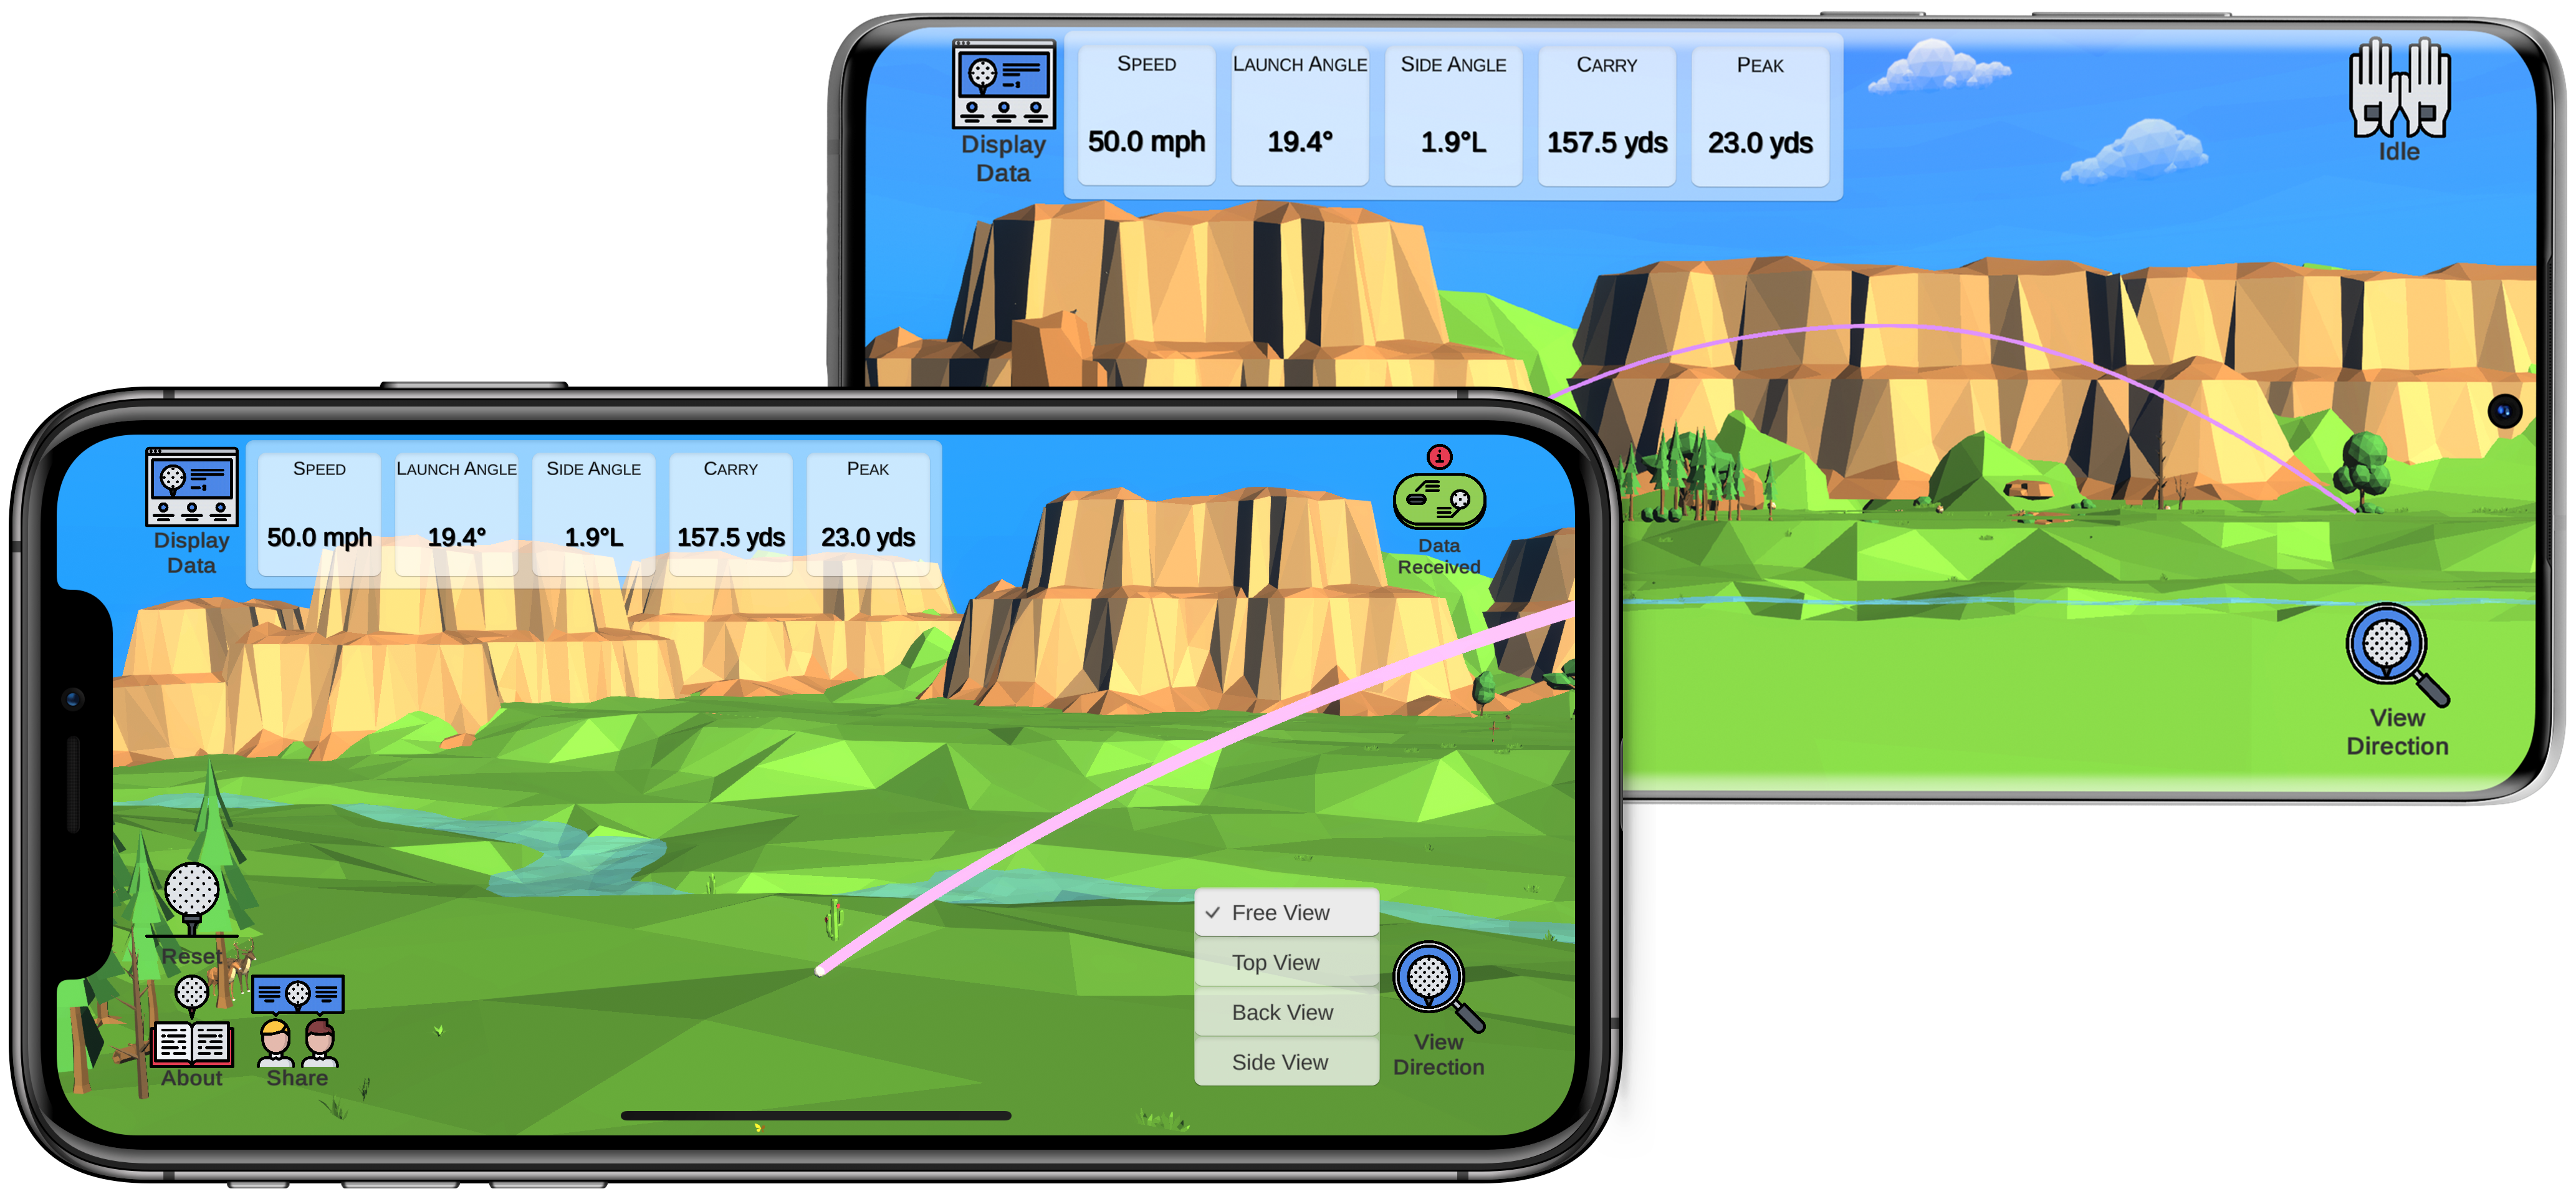
\includegraphics[width=\textwidth]{figure/mockup.png}
    \caption{Graphical user interface of the front-end application}
     \label{fig:mockup}
\end{figure}

\section{Discussion}
With our easy to use mobile app, golfers can not only track the trajectory of any shot but also share their best shots with friends on social media. But there are still some limitations. The current application we have developed is personal game, not available for multiplayer to compare and rank their shot results. Besides that, the app will not give reasonable suggestions to help improve the ball skill based on the simulation result. 

Also, the prediction error of the carry and peak is up to 8$\%$. There are two main reasons for errors. One is the noise in radar system. Three main types of noise can be noise temperature in receivers, multipath reflections, and cluster caused by the disturbance signal returned by other surrounding objects (\cite{martin2012evaluation}). The other one is the accuracy of prediction model. An appropriate model for determining spin rate is needed.


\section{Conclusions and Recommendations}
This report describes the design, development and results of testing of the animation visualization system for the golf flight trajectory. 
In this system, two sets of IVS-565 radars can correctly monitor the Doppler effect of moving objects. Through specially designed amplification, filtering, power supply, level shifter and ADC circuit, the radar signal can be correctly converted into a digital signal that can be read by the Raspberry Pi.

The back-end system equipped on the Raspberry Pi has been proven to run autonomously. The system samples the radar signal at a speed of 20ksps. By adopting the phase-comparison monopulse method, this system can successfully analyse the moving object, and theoretically able to realize the analyse the launch speed and angle of the golf ball.
By establishing a kinematic model of golf ball characteristics using the analysed data, the flight trajectory of the golf ball can be successfully predicted. Finally, the Bluetooth low energy transmission module can stably transmit the flight trajectory data to a smartphone and present the trajectory to the user in real-time with a multi-angle 3D animation.

Due to the restrictions, the radar system and the kinematics model are not able to be calibrated with real golf shots. The lack of golf shot data makes each module of the system has to be tested separately. Due to the limited cooperation method, the hardware part was developed separately, which eventually resulted in a larger circuit.

In the future development, through field testing and calibration of the radar and kinematics model for the golf ball, the stability of the system can be guaranteed, the accuracy of the trajectory simulation can be significantly improved, and eventually verify the predicted flight trajectory of the golf ball. Since the front-end visualization application is based on the Unity engine, the application can easily add functionality related to social interaction and can be extended to AR or VR through further development. In addition, by calibrating the system to different objects, the system can theoretically visualize the flight trajectories of other balls.

\section{Acknowledgements}
We would like to thank Prof. William for giving us the opportunity to complete such an exciting project at this unusual year. Also, we would like to thank the contributors of the open-source software. The software part of the project is based on many open source projects, and the realization of the project is inseparable from the open-source community. Finally, thanks to all of our team members for helping and learning from each other and working together to complete all the work.

\newpage
\section{References}
\printbibliography[heading=none]


\section{Appendices/Supplementary Material}

\end{document}
